\begin{frame}{Game setup and data extraction}
\begin{itemize}
\item Basic game setup
\begin{itemize}
\item 2 teams: blue and purple
\item 10 summoners: 5 on each team
\item Summoner(player): \{level, champion, summoner spells, runes, masteries\}
\item Champion: \{level, 1 passive, 3 abilities, 1 ulti, items, lane\}
\item Lanes: \{top, middle, jungle, bottom\}
\end{itemize}
\end{itemize}
\end{frame}
\begin{frame}{Champion example}
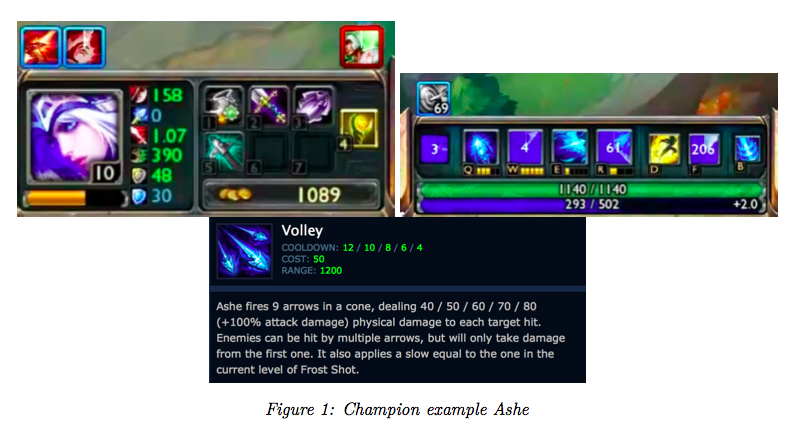
\includegraphics[scale=0.4]{leagueoflegends/ashe}
\end{frame}
\begin{frame}{Match objectives}
\begin{itemize}
\item Nexus: 2 (1 for each team)
\item Inhibitor: 6 (3 for each team)
\item Tower: 22 (11 for each team)
\item Baron: 1
\item Dragon: 1 
\item Gold and experience
\item Killing enemies, minions and monsters
\end{itemize}
\end{frame}
\begin{frame}{The map}
\centering
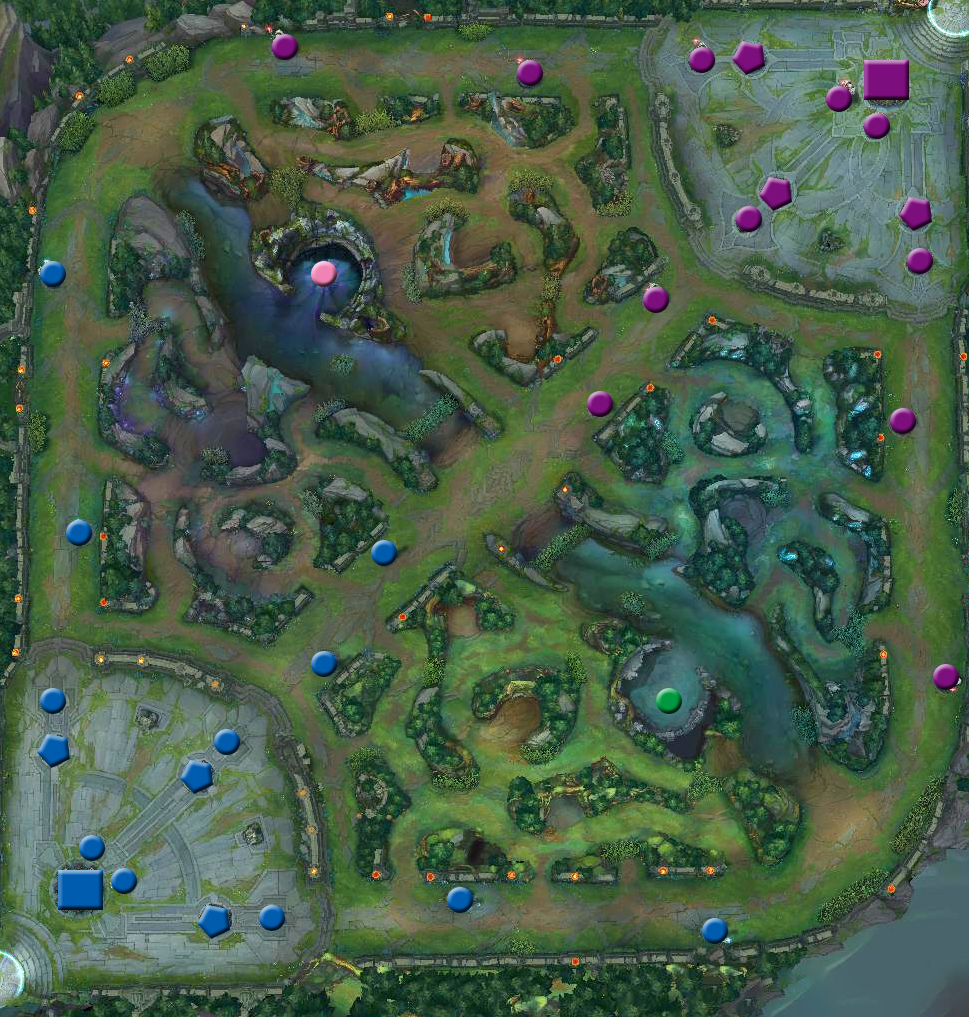
\includegraphics[scale=0.2]{img/kent/lolmap.jpg}
\end{frame}
\begin{frame}{API and data}
\begin{itemize}
\item Riot games API
\begin{itemize}
\item All match data is available through riot games api.
\item Website: https://developer.riotgames.com/
\item Path: /api/lol/\{region\}/v2.2/match/\{matchId\}
\item Path parameters: \{region, matchid\}
\item Query parameter: \{includeTimeline\}
\item Format: Json
\end{itemize}
\end{itemize}
\end{frame}
\begin{frame}{Data object example}
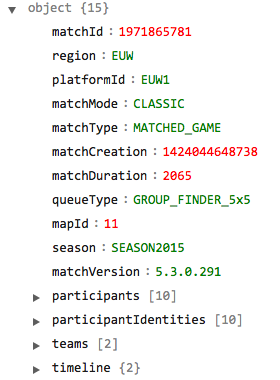
\includegraphics[scale=0.5]{leagueoflegends/gameobject}
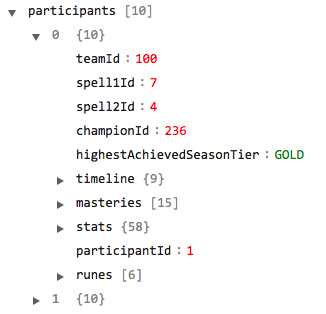
\includegraphics[scale=0.5]{leagueoflegends/participant}
\end{frame}
\begin{frame}{Data filtering}
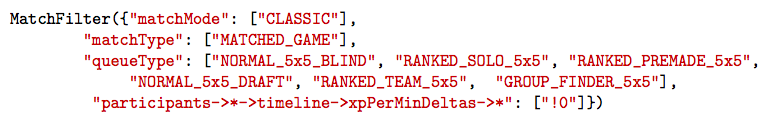
\includegraphics[scale=0.4]{leagueoflegends/mf}
\end{frame}
